\section*{Supplementary Methods and Results}

This document reports the saved extended analyses that support, but do not enlarge, the
claims in the main manuscript. Patient-level uncertainty and repeated tile-sampling
variation are kept distinct. Missing or unevaluable outcomes were never treated as negative
labels, and all endpoint names retain their source definitions.

\noindent\textbf{Abbreviations.} CONCH denotes CONtrastive learning from Captions for
Histopathology; NADT denotes neoadjuvant androgen-deprivation therapy; PANDA denotes
Prostate cANcer graDe Assessment; TCGA-PRAD denotes The Cancer Genome Atlas prostate
adenocarcinoma cohort; and TCGA-CDR denotes the TCGA Pan-Cancer Clinical Data Resource.
Area under the receiver operating characteristic curve (AUROC), time-dependent area under
the curve (td-AUC), concordance index (C-index), integrated Brier score (IBS),
progression-free interval (PFI), progression-free survival (PFS), disease-free survival
(DFS), hematoxylin and eosin (H\&E), copy-number alteration (CNA), confidence interval
(CI), and 256-bit Secure Hash Algorithm (SHA256) are used below. Gene/protein symbols are
expanded as follows: phosphatase and tensin
homolog (PTEN), speckle type BTB/POZ protein (SPOP), androgen receptor (AR), tumor protein
p53 (TP53), RB transcriptional corepressor 1 (RB1), serine peptidase inhibitor Kazal type 1
(SPINK1), ETS variant transcription factors 1 and 4 (ETV1 and ETV4), and ETS transcription
factor ERG (ERG). The post-hoc Cox recurrence-risk score called ``marker 7'' in legacy
artifacts is termed the post-hoc recurrence risk signal here.
CH, EJ, G9, HC, KK, and YL are deidentified source institution codes rather than expanded
institution names.

\noindent Supplementary Table~\ref{tab:supp-endpoint-hierarchy} records the complete
audited endpoint hierarchy without renaming reconstructed outcomes as official PFI.

\begingroup
\small
\begin{longtable}{@{}p{0.06\textwidth}p{0.12\textwidth}p{0.38\textwidth}p{0.35\textwidth}@{}}
\caption{Endpoint hierarchy retained from the audited source. Rows E01--E02 are primary frozen-score qualification, E03 is secondary held-out clinical increment, and E04--E05 are exploratory recurrence analyses. The metric column states the estimand used for each endpoint class; hierarchy levels are not interchangeable.}
\label{tab:supp-endpoint-hierarchy}\\
\toprule
ID & Hierarchy & Endpoint & Primary metric \\
\midrule
\endfirsthead
\toprule
ID & Hierarchy & Endpoint & Primary metric \\
\midrule
\endhead
E01 & primary & continuous marker qualification & patient Spearman rho \\
E02 & primary & binary marker qualification & patient AUROC \\
E03 & secondary & PTEN/AR held-out increment & delta AUROC or delta R2 \\
E04 & exploratory & reconstructed with-tumor endpoint & C-index; td-AUC; IBS; calibration \\
E05 & exploratory & strict recurrence-only endpoint & C-index; td-AUC \\
E06 & exploratory & TCGA-CDR PFS & C-index; td-AUC; landmark AUC \\
E07 & exploratory & TCGA-CDR DFS & C-index; td-AUC; landmark AUC \\
E08 & exploratory & official TCGA-CDR PFI & C-index; endpoint concordance \\
E09 & secondary & 3-year and 5-year landmark & landmark C-index/AUROC \\
\bottomrule
\end{longtable}
\endgroup


The hierarchy distinguishes what each analysis can answer. E01--E02 qualify frozen
continuous and binary marker scores, E03 asks whether PTEN or AR adds held-out information
beyond grade, and E04--E05 are exploratory recurrence analyses with different event
definitions. Consequently, a result in an exploratory recurrence row cannot be used to
upgrade a primary marker claim, and agreement between two endpoint fields does not erase
their declared provenance.

\subsection*{The complete 17-test family}

This subsection enumerates the complete multiplicity family so that the main-text findings
can be interpreted against all saved discovery-family tests rather than a selected subset.

The multiplicity family contained 13 marker hypotheses and four nested/refit confounder
audits. Continuous marker hypotheses used two-sided Spearman tests, binary hypotheses used
two-sided Mann--Whitney tests, and the refit-permutation audit used the saved one-sided
test for positive improvement. Benjamini--Hochberg false-discovery-rate adjustment was applied
jointly to these 17 rows. External or cross-encoder evaluations of an already counted
hypothesis were qualification checks rather than additional discovery-family rows.

\begingroup
\small
\begin{longtable}{@{}p{0.38\textwidth}p{0.14\textwidth}rrr@{}}
\caption{Complete saved 17-row revision-analysis multiplicity family. Effects and probability values are copied from the audited source; $q$ is the Benjamini--Hochberg value.}
\label{tab:supp-family}\\
\toprule
Test & Metric & Effect & $p$ & $q$ \\
\midrule
\endfirsthead
\toprule
Test & Metric & Effect & $p$ & $q$ \\
\midrule
\endhead
\textcircled{1} NADT H\&E -> Gleason & Spearman rho & 0.478 & 0.00207 & 0.00703 \\
\textcircled{2} NADT H\&E -> Phenotype & Spearman rho & 0.8 & $9.63\times10^{-10}$ & $1.64\times10^{-8}$ \\
\textcircled{3} NADT ERG -> Gleason & Spearman rho & 0.524 & 0.00061 & 0.00346 \\
\textcircled{4} TCGA-PRAD H\&E -> PTEN loss & AUROC & 0.632 & 0.000562 & 0.00346 \\
\textcircled{5} TCGA-PRAD H\&E -> SPOP mutation & AUROC & 0.519 & 0.742 & 0.788 \\
\textcircled{6} TCGA-PRAD H\&E -> AR score & Spearman rho & 0.195 & 0.00122 & 0.0052 \\
TCGA-PRAD H\&E -> TP53 mutation & AUROC & 0.485 & 0.835 & 0.835 \\
TCGA-PRAD H\&E -> TP53 CNA loss & AUROC & 0.562 & 0.0981 & 0.208 \\
TCGA-PRAD H\&E -> RB1 CNA loss & AUROC & 0.536 & 0.363 & 0.441 \\
TCGA-PRAD H\&E -> SPINK1 high & AUROC & 0.618 & 0.152 & 0.288 \\
TCGA-PRAD H\&E -> ETV1 altered & AUROC & 0.429 & 0.245 & 0.347 \\
TCGA-PRAD H\&E -> ETV4 altered & AUROC & 0.687 & 0.023 & 0.0559 \\
TCGA-PRAD H\&E -> ERG fusion status & AUROC & 0.526 & 0.458 & 0.519 \\
PTEN / grade-only & AUROC change & 0.0195 & 0.203 & 0.314 \\
AR / grade-only & R-squared change & 0.0044 & 0.176 & 0.299 \\
Post-hoc recurrence risk / grade-only & C-index change & 0.0619 & 0.01 & 0.0283 \\
Post-hoc recurrence risk / fully adjusted & C-index change & 0.00163 & 0.305 & 0.399 \\
\bottomrule
\end{longtable}
\endgroup


Supplementary Table~\ref{tab:supp-family} reports every row in the saved 17-row
revision-analysis multiplicity family; no selected subset is presented as the family.

The family records the tests as originally defined. Later endpoint-matched, same-patient
and same-bootstrap-draw comparisons are reported below and govern the narrower recurrence
interpretation; they do not retrospectively replace rows in the saved multiplicity family.

\subsection*{Detailed discrimination summaries}

We first expand the cross-cohort grade and phenotype evidence underlying the transportable
state assigned in the main Results.

Supplementary Figure~\ref{fig:supp-discrimination-details} shows the saved aggregate
discrimination and association estimates for grade and phenotype transfer across NADT,
PANDA and PRECISE. No
receiver operating characteristic coordinates were stored for these rows, so curves were
not reconstructed from aggregate values. Missing intervals remain visibly unavailable.

\begin{figure}[htbp]
\centering
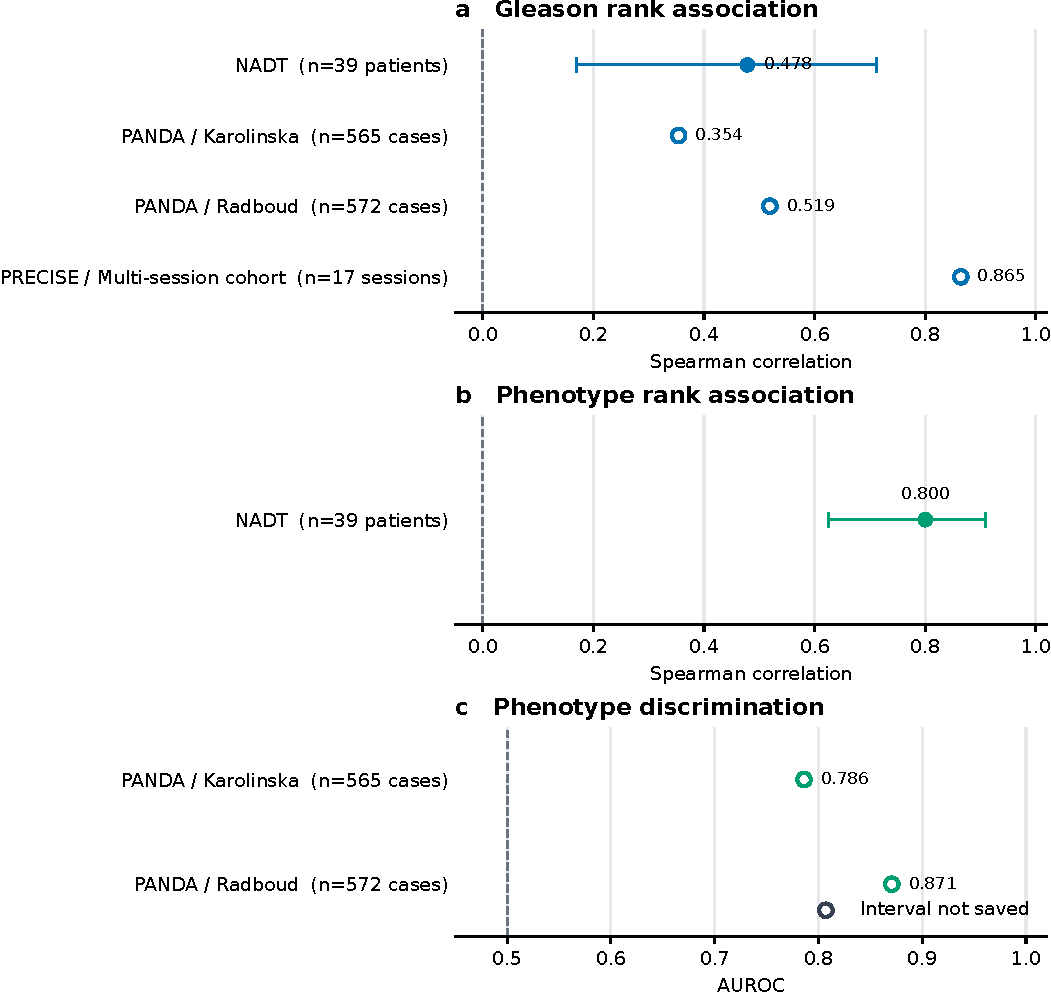
\includegraphics[width=\textwidth]{figures/sfig1_detailed_roc.pdf}
\caption{\textbf{Saved grade and phenotype transport details.} Aggregate patient-,
case-image-, or session-level estimates are separated by metric: \textbf{a}, Gleason
Spearman correlations in NADT-Prostate, PANDA, and PRECISE; \textbf{b}, NADT-Prostate
phenotype Spearman correlation; and \textbf{c}, phenotype AUROC after transfer without
refitting to the Karolinska and Radboud PANDA subsets. Filled points with whiskers show the
saved estimate and patient-bootstrap interval; open points denote estimates for which no
interval was saved. Dashed lines mark $0$ for correlation and $0.5$ for AUROC. Denominators
and analysis units are printed for every row. Unavailable intervals were not treated as zero,
and aggregate statistics were not converted into reconstructed curves.}
\label{fig:supp-discrimination-details}
\end{figure}

The central pattern is directional continuity rather than uniformly precise effect-size
estimation: the NADT-Prostate grade and phenotype signals retain their direction in the
external PANDA subsets and in the PRECISE grade evaluation, but the PANDA and PRECISE rows
without stored intervals do not establish the precision of those effects. Figure S1
therefore supports cross-resource transport of direction while leaving some target-cohort
uncertainty unresolved.

\subsection*{Recurrence endpoints, paired bootstrap and common-source sensitivity}

This subsection tests how the recurrence interpretation changes with endpoint definition,
paired uncertainty estimation, and restriction to a common patient source frame.

The recurrence endpoints were analysed separately. On the 270-patient target frame,
official TCGA-CDR PFI had 42 events and the reconstructed with-tumor endpoint had 57.
Their event agreement was 0.870, Cohen's $\kappa=0.569$, and follow-up-time Spearman
$\rho=0.849$. Official PFI and the cBioPortal TCGA-CDR PFS fields agreed exactly on the
270 common evaluable patients; this identity does not make the separately reconstructed
endpoint equivalent to PFI. Among 192 patients shared with DFS, event agreement was 0.979
and $\kappa=0.835$. Among 220 patients shared with the strict recurrence-only sensitivity,
event agreement was 0.955 and $\kappa=0.564$. These endpoint concordance results come from
\texttt{models/pfi\_endpoint\_concordance.csv}.
Cohen's kappa measures agreement after accounting for agreement expected by chance.

The paired survival analysis used 153 complete cases for each endpoint, with 30
reconstructed-endpoint events and 15 official-PFI events. Every reported model and contrast
requested 2,000 patient-bootstrap resamples. The saved accounting was 2,000 valid and zero
undefined bootstrap replicates (undefined fraction 0) for all 44 model-metric summaries and
all 20 paired contrast-metric summaries. Zero undefined replicates is reported rather than
silently assumed; another dataset could yield undefined concordance or Brier-score draws.

The post-hoc recurrence-risk source-retention audit compared all 60 seed cells on the saved source sets with
the same cells restricted to the common-498 patient intersection. No cell crossed the
C-index null, and all 65 paired contrast directions were preserved. The largest absolute
cell shift was 0.023. This common-498 sensitivity limits source-retention confounding in the
saved grid but does not provide an independent cohort or a causal representation comparison.

Supplementary Figure~\ref{fig:supp-marker7-survival} displays the saved time-dependent AUROC
and calibration summaries for the reconstructed with-tumor endpoint only. This legacy
figure source is not Official TCGA-CDR PFI. Its endpoint identity and analysis frame were
accepted only after the calibration quintiles at both horizons reconciled to the saved
frozen-risk metadata row (270 patients and 57 events). The exploratory marker is not
interpreted as an independently validated prognostic biomarker.

\begin{figure}[htbp]
\centering
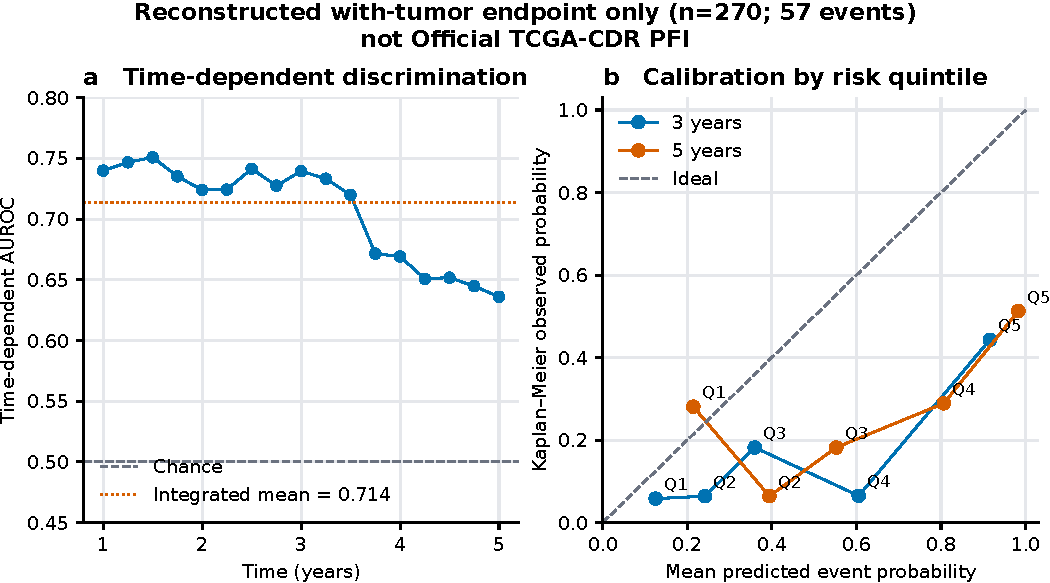
\includegraphics[width=\textwidth]{figures/sfig2_marker7_survival.pdf}
\caption{\textbf{Legacy reconstructed-endpoint post-hoc recurrence-risk summaries.}
Values are rendered from saved legacy sources for the Reconstructed with-tumor endpoint
(270 patients; 57 events), not Official TCGA-CDR PFI. \textbf{a}, Time-dependent AUROC;
the dashed line is chance ($0.5$), and the dotted line is the saved integrated mean over
1--5 years. \textbf{b}, Mean predicted event probability versus Kaplan--Meier observed
probability by risk quintile (Q1--Q5) at 3 and 5 years; the diagonal is ideal calibration and
connecting lines are visual guides across quintiles. The endpoint identity, denominator,
event count, and horizon-specific calibration totals were reconciled to the saved frozen-risk
metadata. Kaplan--Meier is a nonparametric estimate of observed event probability;
calibration compares predicted and observed probabilities; and risk quintiles divide
patients into five ordered groups of predicted risk. This legacy summary is exploratory and
supplies no Official-PFI calibration claim.}
\label{fig:supp-marker7-survival}
\end{figure}

Figure S2 shows that the saved post-hoc score contains time-dependent discrimination and
risk-stratification structure for the reconstructed endpoint. Because both panels use the
same legacy 270-patient frame and reconstructed 57-event definition, they are complementary
descriptions of one exploratory analysis, not two replications and not evidence of Official
PFI calibration.

\clearpage
\subsection*{Full correlated stability analysis}

We next expose the complete sensitivity grid behind the condensed stability decision in the
main manuscript while preserving its correlated, non-confirmatory interpretation.

The saved grid has 72 configurations: six targets, two encoders, two physical scales per
encoder and three tile budgets. Each configuration contains five repeated sampling seeds,
giving 360 correlated seed cells. All settings reused the underlying cohorts and folds.
The five-seed Student-$t$ intervals therefore describe tile-sampling variation, not patient
or population uncertainty. The saved paired-contrast table contains 390 seed-matched
comparisons: 180 native-versus-shared-scale, 90 Virchow-versus-CONCH at shared scale and
120 64-versus-16-tile comparisons.

Supplementary Table~\ref{tab:supp-stability-summary} separates the observed seed range
from the descriptive Student-$t$ interval. Supplementary
Figure~\ref{fig:supp-stability-heatmaps} contains the complete configuration means followed
by the paired contrasts. A setting-specific direction does not identify a causal effect of
encoder, scale or tile count, and the 360 cells are not independent validations.

\begingroup
\small
\captionsetup{justification=raggedright,singlelinecheck=false}
\begin{center}
\begin{minipage}{0.98\textwidth}
\captionof{table}{Global seed-cell ranges and configuration-level null straddling recomputed from all 72 saved configurations. The last two columns count 12 configurations per target and distinguish the observed five-seed range from the descriptive Student-$t$ interval.}
\label{tab:supp-stability-summary}
\centering
\begin{tabular}{@{}lrrrr@{}}
\toprule
Target & Global minimum & Global maximum & Range straddles & $t$-interval contains null \\
\midrule
Gleason & 0.271 & 0.646 & 0/12 & 0/12 \\
Phenotype & 0.845 & 0.965 & 0/12 & 0/12 \\
PTEN & 0.519 & 0.717 & 0/12 & 0/12 \\
AR & 0.136 & 0.297 & 0/12 & 0/12 \\
SPOP & 0.348 & 0.679 & 8/12 & 9/12 \\
Marker 7 & 0.481 & 0.755 & 1/12 & 2/12 \\
\bottomrule
\end{tabular}
\end{minipage}
\end{center}
\endgroup


\clearpage
\begin{figure}[p]
\centering
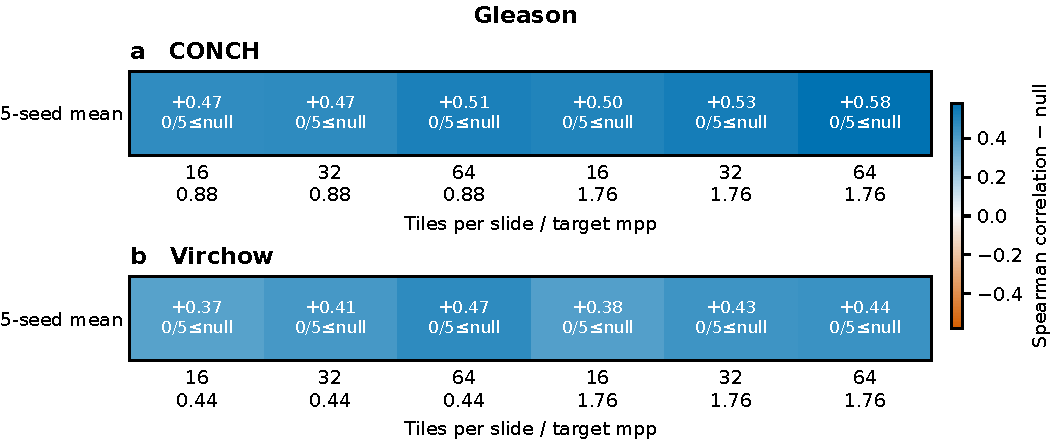
\includegraphics[page=1,width=0.94\textwidth,height=0.29\textheight,keepaspectratio]{figures/sfig3_stability_heatmaps.pdf}
\par\vspace{0.3em}
\includegraphics[page=2,width=0.94\textwidth,height=0.29\textheight,keepaspectratio]{figures/sfig3_stability_heatmaps.pdf}
\caption{\textbf{Complete stability grids and paired contrasts.} Internal pages 1--6
display all 72 validated configuration means from the saved grid, two targets per physical
supplementary page. For each target,
panels \textbf{a--b} are CONCH and Virchow; columns combine 16, 32, or 64 tiles with the
encoder-native physical scale or the shared 1.76~$\mu$m-per-pixel scale. Each cell reports
the five-seed mean minus the marker-specific null and the number of seeds at or below that
null; color is centred at zero separately for each target. Internal pages 7--9 display all 390
seed-matched contrasts: shared 1.76~$\mu$m-per-pixel minus native scale (180), Virchow minus
CONCH at 1.76~$\mu$m per pixel (90), and 64 minus 16 tiles (120). The abscissa is metric
$B-A$ and the dashed line is zero; orange points cross the marker-specific null whereas blue
points remain on the same side. These are descriptive setting checks on reused cohorts and
folds, not independent validations or population-confidence intervals.}
\label{fig:supp-stability-heatmaps}
\end{figure}

\clearpage
\thispagestyle{plain}
\vspace*{\fill}
\begin{center}
\textbf{Supplementary Figure S3 (continued; heatmaps 3--4 of 6)}\\[0.5em]
\includegraphics[page=3,width=0.94\textwidth,height=0.39\textheight,keepaspectratio]{figures/sfig3_stability_heatmaps.pdf}
\par\vspace{0.4em}
\includegraphics[page=4,width=0.94\textwidth,height=0.39\textheight,keepaspectratio]{figures/sfig3_stability_heatmaps.pdf}
\end{center}
\vspace*{\fill}

\clearpage
\thispagestyle{plain}
\vspace*{\fill}
\begin{center}
\textbf{Supplementary Figure S3 (continued; heatmaps 5--6 of 6)}\\[0.5em]
\includegraphics[page=5,width=0.94\textwidth,height=0.39\textheight,keepaspectratio]{figures/sfig3_stability_heatmaps.pdf}
\par\vspace{0.4em}
\includegraphics[page=6,width=0.94\textwidth,height=0.39\textheight,keepaspectratio]{figures/sfig3_stability_heatmaps.pdf}
\end{center}
\vspace*{\fill}

\clearpage
\thispagestyle{plain}
\vspace*{\fill}
\begin{center}
\textbf{Supplementary Figure S3 (continued; scale contrasts)}\\[0.6em]
\includegraphics[page=7,width=0.94\textwidth,height=0.82\textheight,keepaspectratio]{figures/sfig3_stability_heatmaps.pdf}
\end{center}
\vspace*{\fill}

\clearpage
\thispagestyle{plain}
\vspace*{\fill}
\begin{center}
\textbf{Supplementary Figure S3 (continued; encoder contrasts)}\\[0.6em]
\includegraphics[page=8,width=0.94\textwidth,height=0.82\textheight,keepaspectratio]{figures/sfig3_stability_heatmaps.pdf}
\end{center}
\vspace*{\fill}

\clearpage
\thispagestyle{plain}
\vspace*{\fill}
\begin{center}
\textbf{Supplementary Figure S3 (continued; tile-budget contrasts)}\\[0.6em]
\includegraphics[page=9,width=0.94\textwidth,height=0.82\textheight,keepaspectratio]{figures/sfig3_stability_heatmaps.pdf}
\end{center}
\vspace*{\fill}
\clearpage

\subsection*{Target-by-axis evidence coverage}

This subsection makes the synthesis explicit by showing which evidence axis supports,
restricts, or remains unavailable for each target.

The qualification framework deliberately preserves both positive evidence and evidentiary
gaps. Supplementary Figure~\ref{fig:supp-evidence-axis-matrix} shows the complete matrix of
frozen-primary support, cross-cohort transport, clinical increment, site behavior, setting
stability and endpoint fidelity for each target group. A supported cell refers only to the
scope stated for that axis; it does not fill an unevaluated cell elsewhere. Supplementary
Table~\ref{tab:supp-evidence-axis-audit} links every cell to the audited claim source,
states the current interpretation and identifies the evidence required to change that
state.

\begin{figure}[htbp]
\centering
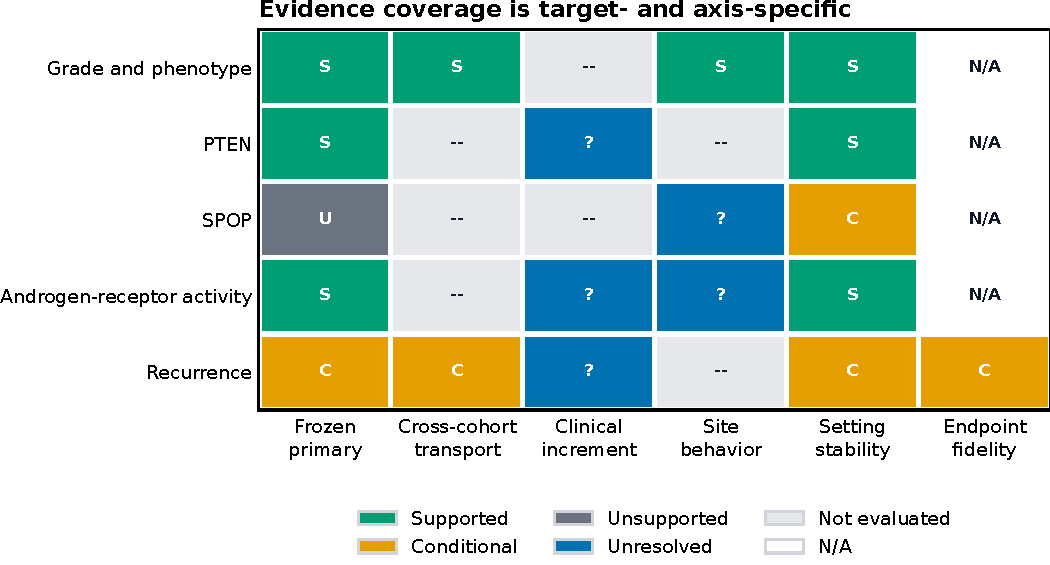
\includegraphics[width=\textwidth]{figures/sfig4_evidence_axis_matrix.pdf}
\caption{\textbf{Target-by-axis evidence coverage.} Each cell records the evidence state
supported by the frozen analyses for one target row and one evidentiary-axis column. Columns
separate frozen-primary support, cross-cohort transport, clinical increment, site behavior,
setting stability, and endpoint fidelity. Cell labels are S (supported), C (conditional),
U (unsupported in the frozen primary design), ? (evaluated but unresolved), -- (not
evaluated), and N/A (not applicable). A supported or conditional cell is bounded to its
named axis and cannot fill another cell; not-evaluated and not-applicable cells are not
negative evidence. The source-linked audit table below provides the claim basis and evidence
needed to change every cell.}
\label{fig:supp-evidence-axis-matrix}
\end{figure}

Read together, Figure S4 and Table S4 show that evidence completeness is target-specific.
Grade and phenotype have the broadest support, including cross-cohort direction; PTEN and
AR have supported within-cohort axes but unresolved or unevaluated clinical and site axes;
SPOP remains unsupported or context-sensitive in the frozen design; and recurrence remains
conditional on representation and endpoint. The matrix is therefore a map of qualified
claims and open gaps, not a scorecard in which supported cells can compensate for missing
ones.

\begingroup
\fontsize{9.5pt}{11pt}\selectfont
\setlength{\tabcolsep}{3pt}
\begin{longtable}{@{}p{0.11\linewidth}p{0.12\linewidth}p{0.12\linewidth}p{0.07\linewidth}p{0.26\linewidth}p{0.26\linewidth}@{}}
\caption{Target-by-axis qualification audit corresponding to main-text Figure 7. Each row links a target-specific evidence state to the audited claim source, states the current evidence, and specifies what evidence would be required to change that state. Not evaluated and not applicable are not negative results.}
\label{tab:supp-evidence-axis-audit}\\
\toprule
Target & Evidence axis & State & Claim & Current evidence & Next evidence needed \\
\midrule
\endfirsthead
\toprule
Target & Evidence axis & State & Claim & Current evidence & Next evidence needed \\
\midrule
\endhead
Grade and phenotype & Frozen primary & supported & C02 & Source-cohort grade and phenotype signals were supported. & Retain the locked source probes and analysis units. \\
Grade and phenotype & Cross-cohort transport & supported & C02 & Direction was retained without refitting in PANDA and was concordant with PRECISE grade evaluation. & Add patient-level uncertainty where source data permit and test further institutions. \\
Grade and phenotype & Clinical increment & not evaluated & C02 & No incremental clinical-covariate claim was defined for these morphology-linked targets. & Define a clinically meaningful reference model before making an increment claim. \\
Grade and phenotype & Site behavior & supported & C02 & Transfer directions were retained at both PANDA institutions; this was not a causal site analysis. & Use site-specific patient-level intervals and acquisition metadata in additional cohorts. \\
Grade and phenotype & Setting stability & supported & C02;C08 & Correlated setting audits retained the transported directions. & Confirm stability on independently sampled patients rather than reused settings. \\
Grade and phenotype & Endpoint fidelity & not applicable & C02 & No time-to-event endpoint was used for these targets. & Not applicable to the present grade and phenotype claims. \\
PTEN & Frozen primary & supported & C03 & The within-TCGA frozen-primary association was above chance. & Repeat the locked evaluation in an external cohort with compatible PTEN labels. \\
PTEN & Cross-cohort transport & not evaluated & C03 & No compatible external PTEN cohort was available in this study. & Acquire an external cohort with target-matched PTEN assays. \\
PTEN & Clinical increment & unresolved & C03 & Held-out increment beyond grade was not established. & Test a locked image increment against grade and fuller clinical covariates in new patients. \\
PTEN & Site behavior & not evaluated & C03 & The manuscript does not establish external site transport for PTEN. & Use a multisite external design with site and acquisition metadata. \\
PTEN & Setting stability & supported & C03;C08 & The within-cohort direction remained above chance across the evaluated grid. & Confirm the direction under independent cohort resampling. \\
PTEN & Endpoint fidelity & not applicable & C03 & PTEN loss was a binary molecular target rather than a clinical time-to-event endpoint. & Not applicable to the present PTEN claim. \\
SPOP & Frozen primary & unsupported in frozen design & C04 & The frozen primary configuration did not support the proposed effect. & Increase target-appropriate sampling without changing the frozen primary interpretation. \\
SPOP & Cross-cohort transport & not evaluated & C04 & No compatible external SPOP cohort was evaluated. & Test a locked probe in an external cohort with mutation labels and tumor-content control. \\
SPOP & Clinical increment & not evaluated & C04 & A grade-independent SPOP increment was not established in the approved analysis set. & Evaluate incremental value with patient-disjoint nested analysis if scientifically justified. \\
SPOP & Site behavior & unresolved & C04 & Defined site intervals included or touched chance and one site was single-class. & Collect larger site-balanced data with assay and acquisition metadata. \\
SPOP & Setting stability & context-sensitive & C04;C08 & The result crossed the null across multiple correlated settings. & Resolve tumor sampling and representation sensitivity in independent data. \\
SPOP & Endpoint fidelity & not applicable & C04 & SPOP mutation was a binary molecular target rather than a clinical time-to-event endpoint. & Not applicable to the present SPOP claim. \\
Androgen-receptor activity & Frozen primary & supported & C05 & The pooled frozen-primary direction was positive. & Retain the pooled result as within-cohort evidence only. \\
Androgen-receptor activity & Cross-cohort transport & not evaluated & C05 & No compatible external androgen-receptor activity cohort was evaluated. & Use an external cohort with a compatible activity assay. \\
Androgen-receptor activity & Clinical increment & unresolved & C05 & Held-out grade-independent increment was not established. & Test a locked incremental model against grade and fuller clinical structure. \\
Androgen-receptor activity & Site behavior & unresolved & C05 & Every stored site-specific interval crossed zero and acquisition effects could not be separated. & Disentangle site from scanner stain preparation and case mix. \\
Androgen-receptor activity & Setting stability & supported & C05;C08 & The positive direction was retained across the correlated setting grid. & Confirm with independently sampled sites and patients. \\
Androgen-receptor activity & Endpoint fidelity & not applicable & C05 & Androgen-receptor activity was a continuous molecular target rather than a time-to-event endpoint. & Not applicable to the present activity-score claim. \\
Recurrence & Frozen primary & context-sensitive & C06 & The transferred post-hoc risk signal depended on representation and endpoint. & Lock the source model before a new independent target-cohort evaluation. \\
Recurrence & Cross-cohort transport & context-sensitive & C06 & LEOPARD-to-TCGA transfer was present in some settings but was not endpoint-invariant. & Test the locked score in an external cohort with a harmonized endpoint. \\
Recurrence & Clinical increment & unresolved & C07 & Full clinical and site comparisons did not establish robust incremental value. & Use an adequately powered same-patient comparison against a clinical reference locked before evaluation. \\
Recurrence & Site behavior & not evaluated & C06;C07 & Site was included in fuller models but site-specific recurrence transport was not isolated. & Evaluate site transport with sufficient events per site. \\
Recurrence & Setting stability & context-sensitive & C06;C08 & Effect size and direction depended on encoder scale and related settings. & Use nested locked model selection and independent validation. \\
Recurrence & Endpoint fidelity & context-sensitive & C06;C07 & Reconstructed recurrence and official PFI produced different evidentiary conclusions. & Harmonize endpoint definitions and retain endpoint-specific reporting. \\
\bottomrule
\end{longtable}
\endgroup


\clearpage

\begin{landscape}
\subsection*{Supplementary evidence atlas}

This subsection consolidates the breadth of the saved evaluation program in forms that are
complementary to the point-and-interval plots in the main manuscript. It does not add new
cohorts, refit a frozen representation, or treat repeated settings as independent
experiments. Supplementary Table~\ref{tab:supp-analysis-frame-inventory} identifies the
analysis unit, denominator, repeated structure, and scientific role of every major evidence
component. Counts from different rows must not be added because patients, slides, folds, and
settings can overlap.

\begingroup
\fontsize{9.5pt}{11pt}\selectfont
\setlength{\tabcolsep}{3pt}
\begin{longtable}{@{}p{0.14\linewidth}p{0.14\linewidth}p{0.14\linewidth}p{0.14\linewidth}p{0.18\linewidth}p{0.20\linewidth}@{}}
\caption{Analysis-frame inventory. Each row identifies the resource, target, analysis unit, saved denominator or repeated structure, and scientific role of one evidence component. Counts must not be summed as independent patients or validations because patients, slides, folds, and settings can overlap across rows.}
\label{tab:supp-analysis-frame-inventory}\\
\toprule
Evidence component & Resource & Target & Analysis unit & Saved frame & Role \\
\midrule
\endfirsthead
\toprule
Evidence component & Resource & Target & Analysis unit & Saved frame & Role \\
\midrule
\endhead
Source fitting & NADT-Prostate & Grade; phenotype & Patient & 39 & Source-cohort probe fitting and patient aggregation \\
External transfer & PANDA Karolinska & Grade; phenotype & Case image & 565; 469 tumor for phenotype & Transfer without target-cohort refitting \\
External transfer & PANDA Radboud & Grade; phenotype & Case image & 572; 483 tumor for phenotype & Transfer without target-cohort refitting \\
Additional grade evaluation & PRECISE & Grade & Imaging session & 17 evaluable sessions & Independent resource and session-level analysis unit \\
Molecular primary & TCGA-PRAD & PTEN; SPOP; AR & Patient & 273 & Frozen pooled association \\
Clinical increment & TCGA-PRAD & PTEN; AR & Patient & 273 & Nested held-out increment beyond grade \\
Site audit & TCGA-PRAD & AR & Slide with patient clustering & 300 slides; 273 patients; 6 sites & Site-specific uncertainty, not a causal scanner analysis \\
Recurrence transfer & TCGA-PRAD & Post-hoc recurrence risk & Patient & 270; 57 reconstructed and 42 Official-PFI events & Endpoint-specific frozen-risk transfer \\
Paired recurrence increment & TCGA-PRAD & Post-hoc recurrence risk & Complete-case patient & 153; 30 reconstructed and 15 Official-PFI events & Same-patient, same-bootstrap-draw model contrasts \\
Correlated setting audit & Multiple source cohorts & Six targets & Configuration and seed cell & 72 configurations; 360 cells; 390 paired contrasts & Sensitivity analysis; cells are not independent validations \\
\bottomrule
\end{longtable}
\endgroup

\end{landscape}

Table S5 demonstrates breadth across cohorts, analysis units, molecular and recurrence
targets, and correlated setting checks. It does not imply that its rows are independent:
the same patient, slide, fold, or saved representation can contribute to more than one row,
so the listed counts must be interpreted within their row-specific analysis frames.

Supplementary Figure~\ref{fig:supp-stability-distributions} exposes all saved paired setting
differences rather than only their global ranges. Each point is one seed-matched comparison,
the violin shows its descriptive distribution, and the embedded box shows the median and
interquartile range. The three panels represent shared-minus-native physical scale,
Virchow-minus-CONCH encoder, and 64-minus-16-tile contrasts. Orange points identify pairs
whose endpoints lie on opposite sides of the marker-specific null; they do not represent
independent hypothesis tests. The complete numerical summaries are reported in
Supplementary Table~\ref{tab:supp-stability-contrast-summary}.

\begin{figure}[htbp]
\centering
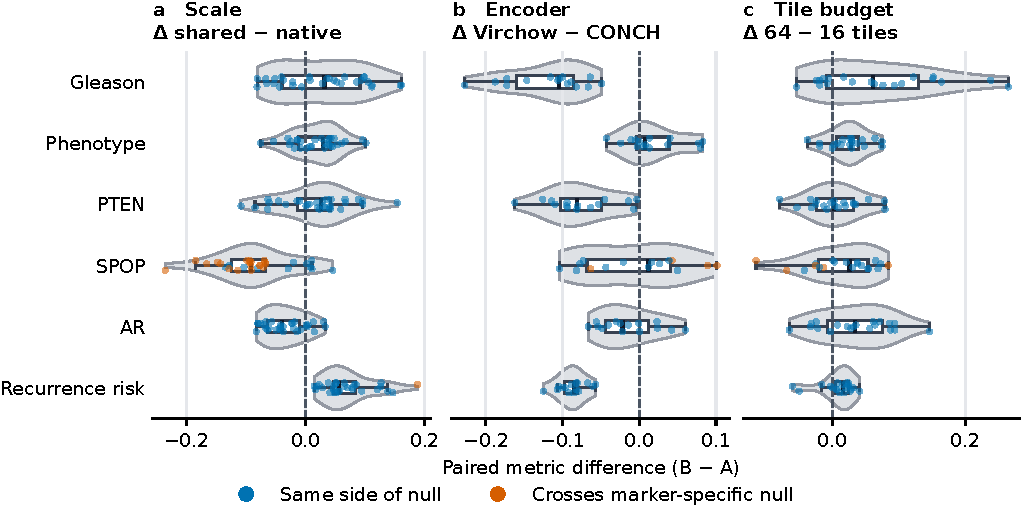
\includegraphics[width=\textwidth]{figures/sfig5_stability_distributions.pdf}
\caption{\textbf{Distributions of all seed-matched stability contrasts.}
\textbf{a}, Shared 1.76-micrometre-per-pixel scale minus each encoder's native scale.
\textbf{b}, Virchow minus CONCH at the shared scale. \textbf{c}, 64 minus 16 sampled tiles
per slide. Horizontal violins show the distribution of saved paired metric differences;
white boxes span the interquartile range, black lines mark medians, and individual dots are
the complete seed-matched contrasts. Blue pairs remain on the same side of the relevant
null and orange pairs cross it. Positive values favor the second-named setting under the
displayed B-minus-A convention. All pairs reuse cohorts and folds and therefore describe
setting sensitivity rather than independent validation evidence.}
\label{fig:supp-stability-distributions}
\end{figure}

\begingroup
\small
\setlength{\tabcolsep}{3pt}
\begin{longtable}{@{}p{0.29\textwidth}p{0.16\textwidth}rrrr@{}}
\caption{Descriptive summary corresponding to Supplementary Figure S5. All 390 seed-matched setting contrasts are partitioned by comparison family and target. Differences are B minus A; medians, interquartile ranges, and null-crossing counts summarize correlated sensitivity comparisons rather than independent replicates or hypothesis tests.}
\label{tab:supp-stability-contrast-summary}\\
\toprule
Comparison & Target & Pairs & Median & Interquartile range & Null crossings \\
\midrule
\endfirsthead
\toprule
Comparison & Target & Pairs & Median & Interquartile range & Null crossings \\
\midrule
\endhead
Shared 1.76 mpp minus native & Gleason & 30 & +0.032 & -0.039 to +0.092 & 0/30 \\
Shared 1.76 mpp minus native & Phenotype & 30 & +0.029 & -0.012 to +0.043 & 0/30 \\
Shared 1.76 mpp minus native & PTEN & 30 & +0.026 & -0.013 to +0.043 & 0/30 \\
Shared 1.76 mpp minus native & AR & 30 & -0.039 & -0.063 to -0.010 & 0/30 \\
Shared 1.76 mpp minus native & SPOP & 30 & -0.091 & -0.124 to -0.067 & 19/30 \\
Shared 1.76 mpp minus native & Recurrence risk & 30 & +0.056 & +0.047 to +0.084 & 1/30 \\
Virchow minus CONCH at 1.76 mpp & Gleason & 15 & -0.105 & -0.160 to -0.085 & 0/15 \\
Virchow minus CONCH at 1.76 mpp & Phenotype & 15 & +0.008 & -0.004 to +0.039 & 0/15 \\
Virchow minus CONCH at 1.76 mpp & PTEN & 15 & -0.081 & -0.102 to -0.049 & 0/15 \\
Virchow minus CONCH at 1.76 mpp & AR & 15 & -0.022 & -0.044 to +0.012 & 0/15 \\
Virchow minus CONCH at 1.76 mpp & SPOP & 15 & +0.012 & -0.068 to +0.041 & 4/15 \\
Virchow minus CONCH at 1.76 mpp & Recurrence risk & 15 & -0.085 & -0.098 to -0.080 & 0/15 \\
64 minus 16 tiles & Gleason & 20 & +0.061 & -0.009 to +0.129 & 0/20 \\
64 minus 16 tiles & Phenotype & 20 & +0.028 & +0.007 to +0.039 & 0/20 \\
64 minus 16 tiles & PTEN & 20 & +0.003 & -0.024 to +0.032 & 0/20 \\
64 minus 16 tiles & AR & 20 & +0.034 & -0.007 to +0.075 & 0/20 \\
64 minus 16 tiles & SPOP & 20 & +0.026 & -0.021 to +0.054 & 5/20 \\
64 minus 16 tiles & Recurrence risk & 20 & +0.017 & +0.005 to +0.024 & 0/20 \\
\bottomrule
\end{longtable}
\endgroup


Figure S5 and Table S6 make the heterogeneity behind the condensed stability decision
visible. Grade, phenotype, PTEN, and AR have no null-crossing pairs in the saved contrast
families, whereas SPOP contains crossings for scale, encoder, and tile-budget comparisons.
The recurrence-risk signal has one scale crossing and a consistently negative
Virchow-minus-CONCH contrast on this grid. These patterns identify settings that require
qualification; they do not rank encoders causally or turn repeated seeds into independent
experiments.

Supplementary Figure~\ref{fig:supp-endpoint-concordance} separates three notions that can
otherwise be hidden by a single endpoint label: event agreement, chance-corrected agreement,
and follow-up-time rank correlation. The event-pair composition shows where apparent
agreement arises from shared non-events and where the event indicators disagree. Exact
agreement between Official TCGA-CDR PFI and the saved TCGA-CDR PFS fields reflects their
source-field identity in this analysis; it is not an independent replication. Conversely,
high raw agreement with other endpoints does not make their event definitions equivalent.

\begin{figure}[htbp]
\centering
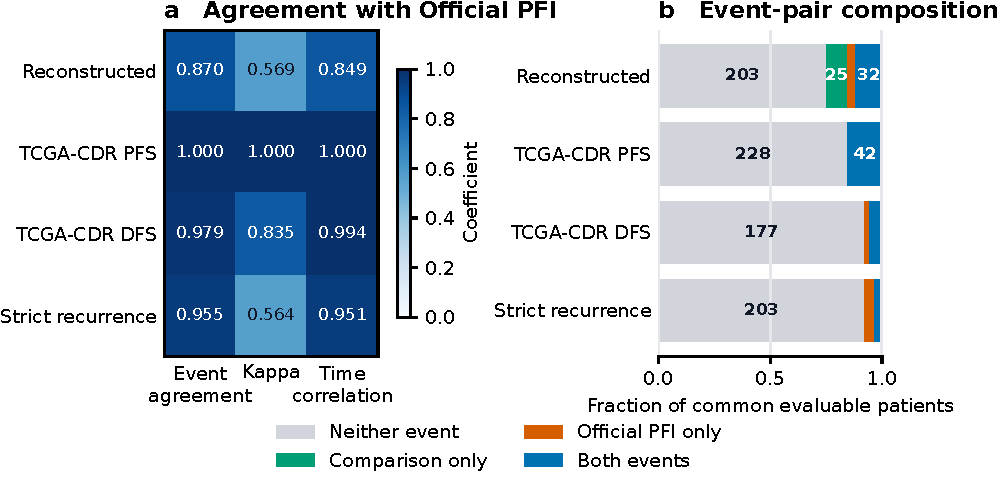
\includegraphics[width=\textwidth]{figures/sfig6_endpoint_concordance.pdf}
\caption{\textbf{Endpoint concordance relative to Official TCGA-CDR progression-free
interval (PFI).} \textbf{a}, Heatmap of raw event agreement, Cohen's kappa, and Spearman
correlation of follow-up times among common evaluable patients. Cohen's kappa adjusts event
agreement for agreement expected by chance. \textbf{b}, Composition of the corresponding
event pairs; numbers within sufficiently large segments are patient counts. Grey denotes
neither endpoint recording an event, green the comparison endpoint only, orange Official
PFI only, and blue both endpoints. Differences in evaluable frames and event definitions
remain part of the interpretation.}
\label{fig:supp-endpoint-concordance}
\end{figure}

\begin{table}[htbp]
\centering
\small
\caption{Saved endpoint concordance corresponding to Supplementary Figure S6, with Official TCGA Pan-Cancer Clinical Data Resource progression-free interval (PFI) as the reference. Common N is the shared evaluable frame; event counts are Official PFI/comparison; agreement is raw event agreement, kappa is chance-corrected event agreement, and time rho is Spearman follow-up-time correlation.}
\label{tab:supp-endpoint-concordance}
\begin{tabular}{@{}lrrrrr@{}}
\toprule
Comparison endpoint & Common N & Events & Agreement & Kappa & Time rho \\
\midrule
Reconstructed with-tumor & 270 & 42/57 & 0.870 & 0.569 & 0.849 \\
TCGA-CDR PFS & 270 & 42/42 & 1.000 & 1.000 & 1.000 \\
TCGA-CDR DFS & 192 & 15/11 & 0.979 & 0.835 & 0.994 \\
Strict recurrence-only & 220 & 17/7 & 0.955 & 0.564 & 0.951 \\
\bottomrule
\end{tabular}
\end{table}


Figure S6 and Table S7 show why raw agreement alone is insufficient. The exact Official-PFI
and TCGA-CDR-PFS row reflects identical saved source fields in this analysis, while the
reconstructed and strict-recurrence rows combine high raw agreement with only moderate
chance-corrected agreement. Recurrence conclusions are therefore reported by endpoint
rather than pooled under a single label.

\clearpage

\subsection*{AR site uncertainty and SPOP detectable-effect calculations}

We then provide the detailed checks that bound the site-specific AR interpretation and the
effect sizes that the frozen SPOP analysis was positioned to detect.

The AR site audit estimated slide-level Spearman correlations and used patient-cluster
bootstrap intervals. Six leave-one-site-out rows were available: CH, $-0.128$
($-0.561$ to 0.350); EJ, 0.127 ($-0.121$ to 0.363); G9, 0.195 ($-0.258$ to 0.598);
HC, 0.217 ($-0.072$ to 0.471); KK, 0.265 ($-0.087$ to 0.558); and YL, 0.227
($-0.135$ to 0.541). Every site-specific interval included zero. The positive pooled
patient-level estimate therefore did not establish transport at any individual site, and
the data did not identify scanner or stain as a cause.

For SPOP, the saved planning calculation used 29 positive and 244 negative patients, a
two-sided $\alpha=0.05$ test and a fixed-score Hanley--McNeil normal approximation. The
minimum detectable AUROC was 0.661 at 80\% power and 0.685 at 90\% power. These values omit
probe-training uncertainty, out-of-fold dependence, site heterogeneity, setting selection
and multiplicity. They are planning approximations, not effect-exclusion bounds; they do
not show that smaller effects or sampling dilution are absent. In this calculation,
``minimum detectable'' means the smallest assumed AUROC that reaches the specified power
under the stated assumptions, not the smallest biologically possible effect.

\subsection*{Provenance and reproducibility scope}

The final subsection identifies the saved records supporting computational traceability and
distinguishes that traceability from external or clinical validation.

The extended results were read from saved CSV sources rather than recomputed from remembered
values. Stability lineage is recorded in \path{models/stability_run_manifest.csv} and
\path{models/stability_qc_report.json}; recurrence lineage is recorded in the paired
survival and common-source run configurations and manifests; AR and SPOP source hashes are
recorded in \path{models/ar_spop_evidence_manifest.csv}. The manuscript source tables
and figure renderers are linked by the submission figure manifest. The PRECISE clinician
review source was kept immutable and its SHA256 was checked against
\texttt{c1dd522b}\allowbreak\texttt{4ff4f233}\allowbreak
\texttt{b3a23630}\allowbreak\texttt{bf9074da}\allowbreak
\texttt{881bb7b9}\allowbreak\texttt{145996fc}\allowbreak
\texttt{47c3383a}\allowbreak\texttt{0448d2a3}.
A SHA256 hash is a file fingerprint used to detect byte-level changes, while a manifest is
an inventory linking named inputs, code, configurations and outputs.

These records support auditability of the saved analyses. They do not establish population
prevalence, whole-slide diagnostic performance, external molecular validation or clinical
utility.
